% -*- LaTeX -*-
% -*- coding: utf-8 -*-
%
% ~~~~~~~~~~~~~~~~~~~~~~~~~~~~~~~~~~~~~~~~~~~~~~~~~~~~~~~~~~~~~~~~~~~~~~~~~~~~~~
%
%                             michael a.g. aïvázis
%                      california institute of technology
%                      (c) 1998-2010  all rights reserved
%
% ~~~~~~~~~~~~~~~~~~~~~~~~~~~~~~~~~~~~~~~~~~~~~~~~~~~~~~~~~~~~~~~~~~~~~~~~~~~~~~
%

\lecture{Programming NVidia GPUs with CUDA}{20100129}

% --------------------------------------
% template
\begin{frame}[fragile]
%
  \frametitle{Hybrid architectures}
%
  \begin{itemize}
%
  \item recall the layout of SIMD machines
    \begin{itemize}
    \item a large number of small, special purpose processors
    \item a single ``controller'' manages the instruction stream
      \begin{itemize}
      \item each processor executes the same instruction on its local data
      \item may be able to specify which processors are active/idle
      \end{itemize}
    \end{itemize}
    \begin{figure}
      \centering
      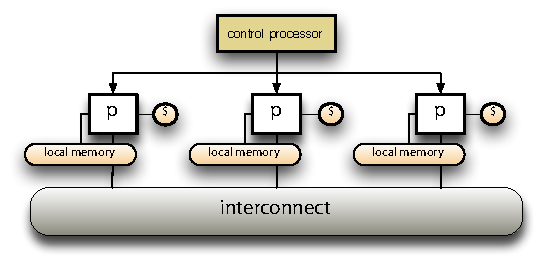
\includegraphics[width=.50\linewidth]{figures/simd.pdf}
      \label{fig:simd}
    \end{figure}
%
  \item modern hybrid systems based on GPUs have somewhat more elaborate architectures
    \begin{itemize}
      \item multi-tier memory layouts
      \item large core counts per board
      \item elaborate access rules that enable the hardware to be very fast
      \item recent ones finally support double precision floating point arithmetic
      \item broadly available -- it's in your graphics card, thanks to video gaming
    \end{itemize}
%
  \end{itemize}
%
\end{frame}

% --------------------------------------
% CUDA architecture
\begin{frame}[fragile]
%
  \frametitle{nVidia GPU architecture}
%
  \begin{itemize}
  \item The GPU boards are hosted by a conventional processor
    \begin{itemize}
    \item connected through PCI Express, which is the limiting factor in moving data to and
      from the device memory
    \end{itemize}
  \item computing power and memory configurations vary from
    \begin{itemize}
    \item a single 2-core GPU with 128M of memory on older video cards
    \item to 30 $\times$ 8-core SIMTs with 4G of memory on the Tesla C1060
      \begin{itemize}
      \item 240 cores; peak: 933 Gflops single precision, 78 Gflops double precision
      \item \href{rivulet.cacr.caltech.edu} has four such boards
      \end{itemize}
    \end{itemize}
  \end{itemize}  
  
%
  \begin{figure}
    \centering
    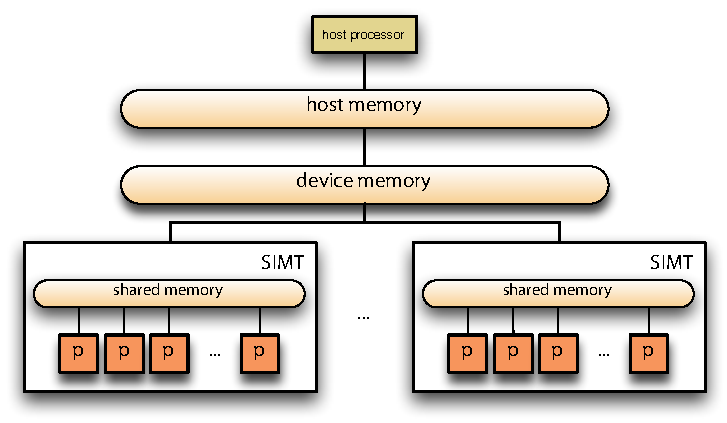
\includegraphics[width=0.75\linewidth]{figures/cuda-architecture.pdf}
    \label{fig:simd}
  \end{figure}
%
\end{frame}

% --------------------------------------
% getting started
\begin{frame}[fragile]
%
  \frametitle{Getting started}
%
  \begin{itemize}
%
  \item getting the drivers, tools and code samples
    \begin{itemize}
    \item visit \href{http://nvidia.com/cuda}
    \end{itemize}
%
  \item compiling and linking
    \begin{itemize}
    \item \cc\ for CUDA: a few extensions
    \item source is a mixture of the code that runs on the host and the {\em kernels} that run
      on the \identifier{GPU}
    \item there are restrictions on what kind of code you can include in a kernel
    \item \identifier{nvcc} is the special compiler and linker
    \end{itemize}
%
  \item staging and launching
    \begin{itemize}
    \item the resulting executable runs on the host
    \item launches threads on the GPU through special statements
    \end{itemize}
%
  \item the emulator
    \begin{itemize}
    \item the SDK comes with a software emulator
    \item extremely useful for debugging
    \end{itemize}
%
  \item special hardware
    \begin{itemize}
    \item your video card
    \item Tesla boards
    \end{itemize}
%
  \end{itemize}
%
\end{frame}

% --------------------------------------
% sanity check
\begin{frame}[fragile]
%
  \frametitle{Sanity check}
  \label{slide:sanity-cuda}
%
  \begin{C}[basicstyle=\tt\bfseries\tiny]
// memxchng.cu: making sure the compiler and cuda runtime are accessible
#include <cuda.h>
#include <assert.h>

int main(int argc, char* argv[]) {
    const int N = 12;
    // allocate some buffers on the host
    float *send_host = (float *) malloc(N*sizeof(float));
    float *recv_host = (float *) malloc(N*sizeof(float));
    // allocate matching ones on the device
    float *send_device, *recv_device;
    cudaMalloc((void **) &recv_device, N*sizeof(float));
    cudaMalloc((void **) &send_device, N*sizeof(float));
    // and initialize the host data
    for (int i=0; i<N; i++) {
        send_host[i] = 2.0f + i*i;
        recv_host[i] = 0.0f;
    }
    // send the data from the host to the device
    cudaMemcpy(recv_device, send_host, N*sizeof(float), cudaMemcpyHostToDevice);
    // move the data in device memory
    cudaMemcpy(send_device, recv_device, N*sizeof(float), cudaMemcpyDeviceToDevice);
    // get it back on the host
    cudaMemcpy(recv_host, send_device, N*sizeof(float), cudaMemcpyDeviceToHost);
    // check the result
    for (int i=0; i<N; i++) {
      assert(send_host[i] == recv_host[i]);
    }
    // free the buffers;
    free(send_host); free(recv_host);
    cudaFree(send_device); cudaFree(recv_device);

    return 0;
}
  \end{C}
%
\end{frame}

% --------------------------------------
% the execution model
\begin{frame}[fragile]
%
  \frametitle{The execution model}
%
  \begin{itemize}
%
  \item \identifier{nvcc} splits the source code into two parts
    \begin{itemize}
    \item the code that runs on the host
    \item the device {\em kernel}, the code that runs of the GPU 
      \begin{itemize}
      \item built out of specially marked subroutines in the program
      \end{itemize}
    \end{itemize}
  \item the program is launched on the host and runs sequentially
  \item at specific points in the code, the program
    \begin{itemize}
    \item launches the kernel and runs it on the GPU by many threads in parallel
    \item the host continues on without blocking 
    \item until it encounters some blocking call to the CUDA runtime
    \end{itemize}
%
  \item the execution context is specified by organizing
    \begin{itemize}
    \item groups of threads in {\em blocks}
    \item groups of blocks in {\em grids}
    \item blocks are scheduled and executed in arbitrary order
      \begin{itemize}
      \item in {\em warps}: 32 SIMD threads at a time (on currently available devices)
      \end{itemize}
    \end{itemize}
%
  \item at runtime, each thread is given
    \begin{itemize}
    \item \identifier{threadIdx}: its own thread id
    \item \identifier{blockIdx}: the id of the block of active threads
    \item \identifier{blockDim}: the geometry of the block of active threads
    \end{itemize}
%
  \end{itemize}
%
\end{frame}

% --------------------------------------
% the memory manipulations
\begin{frame}[fragile]
%
  \frametitle{Adding a bit of work}
  \label{slide:hello-world-cuda}
%
  \begin{C}
// scale.cu: multiply each element in an array by a given float
#include <cuda.h>
#include <assert.h>

// manipulate the host array
void scale_host(float* a, float scale, int N) {
    // loop over all array elements and multiply them by 2 
    for (int i=0; i<N; i++) {
        a[i] *= scale;
    }
    return;
}

// and here is the corresponding code for the GPU
__global__ void scale_device(float* a, float scale, int N) {
    // this thread is responsible for one element of the array
    // compute its offset using the block geometry builtins
    int idx = blockIdx.x * blockDim.x  + threadIdx.x;
    // make sure we don't do go past the last one
    if (idx < N) {
        // do the arithmetic
        a[idx] *= scale;
    }
    return;
}
  \end{C}
%
\end{frame}

% --------------------------------------
% launching the kernel
\begin{frame}[fragile]
%
  \frametitle{Launching the kernel}
  \label{slide:launching-kernel-cuda}
%
  \begin{C}
    . . .
    // send the data from the host to the device
    cudaMemcpy(
        array_dev, send_host, N*sizeof(float), cudaMemcpyHostToDevice);

    // set up the device execution context for our threads
    // each thread will take care of one element
    int blockSz = 4; // 4 threads per block
    // compute the number of blocks needed
    int nBlocks = N/blockSz; 
    // adjust up to make sure we cover the entire array
    if (N % nBlocks) {
        nBlocks++;
    }
    // scale the array on the device
    float scale = 2.0f;
    scale_device <<<nBlocks, blockSz>>> (array_dev, scale, N);
    // scale the input array on the host
    scale_host(send_host, scale, N);

    // get it back on the host
    cudaMemcpy(
        recv_host, array_dev, N*sizeof(float), cudaMemcpyDeviceToHost);
    . . .

  \end{C}
%
\end{frame}

% --------------------------------------
% the Tesla C1060
\begin{frame}[fragile]
%
  \frametitle{Capabilities of the Tesla C1060 board}
%
  \begin{shell}[basicstyle=\tt\bfseries\tiny]

Device 1: "Tesla C1060"
  CUDA Driver Version:                           2.30
  CUDA Runtime Version:                          2.30
  CUDA Capability Major revision number:         1
  CUDA Capability Minor revision number:         3
  Total amount of global memory:                 4294705152 bytes
  Number of multiprocessors:                     30
  Number of cores:                               240
  Total amount of constant memory:               65536 bytes
  Total amount of shared memory per block:       16384 bytes
  Total number of registers available per block: 16384
  Warp size:                                     32
  Maximum number of threads per block:           512
  Maximum sizes of each dimension of a block:    512 x 512 x 64
  Maximum sizes of each dimension of a grid:     65535 x 65535 x 1
  Maximum memory pitch:                          262144 bytes
  Texture alignment:                             256 bytes
  Clock rate:                                    1.30 GHz
  Concurrent copy and execution:                 Yes
  Run time limit on kernels:                     No
  Integrated:                                    No
  Support host page-locked memory mapping:       Yes
  Compute mode:                                  Default
                                                 (multiple host threads can 
                                                 use this device simultaneously)
  \end{shell}
%
\end{frame}

% --------------------------------------
% memory hierarchy
\begin{frame}[fragile]
%
  \frametitle{Memory hierarchy}
%
  \begin{minipage}{.55\linewidth}
    \begin{itemize}
    \item each thread gets
      \begin{itemize}
      \item a set of {\em registers}: really fast but limited memory
      \item memory {\em shared} by all threads in its block
      \item private {\em local} memory allocated from the global address space
      \item access to the device {\em global} memory pool
      \end{itemize}
    \item {\em texture} and {\em constant} memory are beyond scope here
      \begin{itemize}
      \item not really useful for general purpose programming
      \end{itemize}
    \item latency and bandwidth for these memory pools are very different
      \begin{itemize}
      \item the name of the game: resource management
      \item the price to pay for the astronomical performance
      \end{itemize}
    \end{itemize}
  \end{minipage}
 %
  \hfill
  \begin{minipage}{.40\linewidth}
    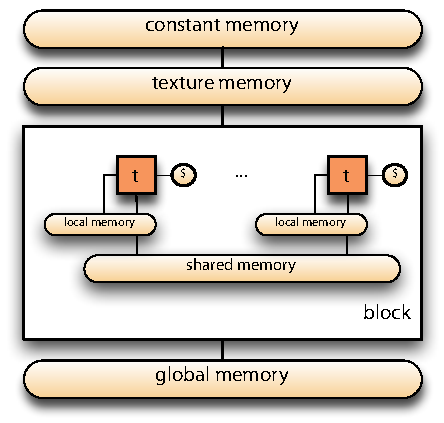
\includegraphics[scale=0.65]{figures/cuda-blocks.pdf}
  \end{minipage}
%
\end{frame}

% --------------------------------------
% summary
\begin{frame}[fragile]
%
  \frametitle{Summary}
%
  \begin{itemize}
%
  \item GPUs brought hybrid programming models back to center stage
    \begin{itemize}
    \item but our parallelization steps don't change
    \item just the balance between fine and coarse grain tasks
    \end{itemize}
%
  \item high performance computing the way it used to be
    \begin{itemize}
    \item resource allocation and management strategies define performance
    \item true enough for sequential, \mpi\ and threaded programs anyway
    \end{itemize}
%
  \item barely scratched the surface here
    \begin{itemize}
    \item let me know if you are interested in pursuing further
    \end{itemize}
%
  \item if you must program in a hybrid model
    \begin{itemize}
    \item why not write multi-threaded host programs
      \begin{itemize}
      \item to take advantage of more devices per host
      \item to overlap calculations on the host and GPU
      \end{itemize}
    \item why not use \mpi\ as well and scale out to multiple nodes
      \begin{itemize}
      \item for some really massive calculations!
      \end{itemize}
    \end{itemize}
%
  \end{itemize}
%
\end{frame}

% end of file 
